The diagram shows three vectors, $\overrightarrow{A}$, $\overrightarrow{B}$, and $\overrightarrow{C}$. All three are in plane with the page; their magnitudes are (respectively) 2, 1, and 3. For each operation below, either draw the results of the identified operations, or (if appropriate) give a best guess as to the value, or (if appropriate) identify the operation as nonsense.

\begin{center}
\begin{tikzpicture}
  \draw[line width=1pt,black,-stealth](-3,0)--(-4.414,1) node[anchor=south west]{$\overrightarrow{A}$};
  \draw[line width=1pt,black,-stealth](0,0)--(0.25,0.97) node[anchor=south west]{$\overrightarrow{B}$};
  \draw[line width=1pt,black,-stealth](3,0)--(6, 0) node[anchor=south west]{$\overrightarrow{C}$};
\end{tikzpicture}
\end{center}

$\overrightarrow{A} + \overrightarrow{B}$

\begin{solution}\
\begin{center}
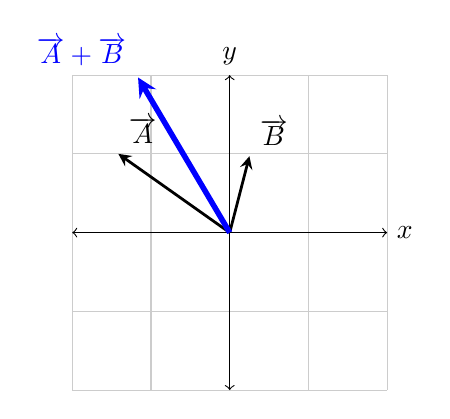
\begin{tikzpicture}
  \draw[thin,gray!40] (-2,-2) grid (2,2);
  \draw[<->] (-2,0)--(2,0) node[right]{$x$};
  \draw[<->] (0,-2)--(0,2) node[above]{$y$};
  \draw[line width=1pt,black,-stealth](0,0)--(-1.414,1) node[anchor=south west]{$\overrightarrow{A}$};
  \draw[line width=1pt,black,-stealth](0,0)--(0.25,0.97) node[anchor=south west]{$\overrightarrow{B}$};
  \draw[line width=2pt,blue,-stealth](0,0)--(-1.164, 1.97) node[anchor=south east]{$\overrightarrow{A}+\overrightarrow{B}$};
\end{tikzpicture}
\end{center}
\end{solution}